\chapter{Discussion}

\begin{center}
    \textit{The results are analyzed and discussed in this chapter. It explores the implications of the findings, identifies limitations, and suggests potential areas for future improvement.}
\end{center}

\section{Temporary Title – Discussion of Results}

WORK IN PROGRESS

The model’s strategy of selecting the most likely move revealed a notable flaw in castling detection. Specifically, castling moves were often misclassified due to the system evaluating each piece movement independently. In many cases, the model assigned a higher confidence score to the rook's move from its original square than to the king’s two-square movement during castling. Consequently, 8 out of 9 misclassifications occurred when the model incorrectly selected the rook’s movement as the intended move, rather than recognizing the castling sequence. A possible solution is to briefly delay the rook’s movement, allowing the king’s two-square move to occur first. This removes ambiguity by ensuring that, at the moment of detection, only a single plausible move is visible—effectively forcing the model to select the castling move rather than misclassifying it as a standalone rook move. \\

Another recurring issue was observed in the form of consistent failure points within specific openings. In several test sets, all 10 games of a given opening failed at the same move number. This pattern suggests that certain positions or board states consistently challenge the model, possibly due to recurring piece configurations or lighting conditions at those points in the game. \\

Additionally, move detection accuracy decreased noticeably along the edges of the board. This limitation appears to result from a combination of factors. First, the board-warping algorithm relies on precise corner detection to accurately map square centers. While the inner squares were typically well-aligned, the outermost squares—particularly near the corners—were more prone to distortion, likely contributing to errors in piece localization. Second, the relatively steep camera angle made it harder to clearly distinguish pieces near the front edge of the board, as those closest to the lens were partially occluded or lacked visible detail. Third, pieces on the far side of the board appeared smaller in the frame, and the inter-square distances in the warped image were reduced. This made it more likely for pieces to be mistakenly assigned to adjacent squares, especially along the tighter edge regions. \\

\subsection{Different gamemodes}

The models job is to find the pieces on the board and then assign them to its respective square. This means as long as you define the starting postion or start fen, that allows you to play any the game from any posistion you want. That means you could start a match mid game or you could play other game modes. The model also has validation so that means it should be able to successfully



Further testing supported these findings. As shown in Figure~\ref{fig:bbox-centers-incorrect}, the bounding boxes along the edges of the board are occasionally misaligned, reinforcing the challenges associated with edge square detection.

\begin{figure}[h!]
    \centering
    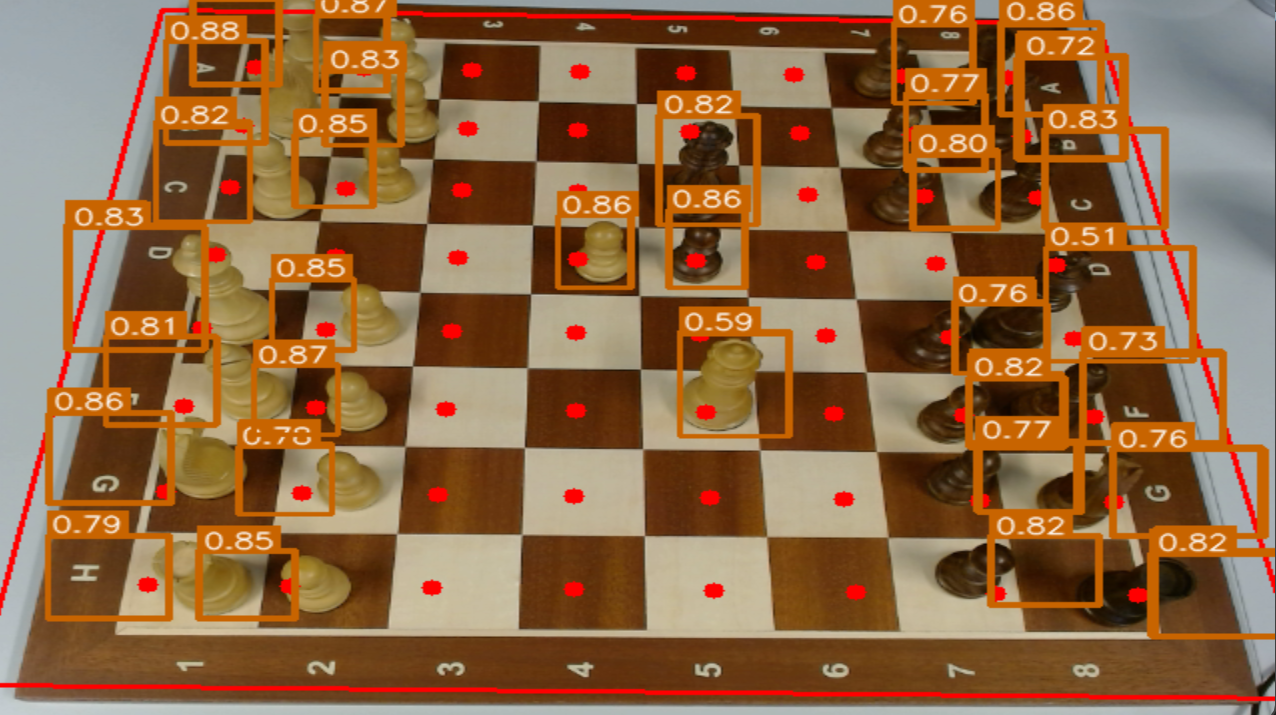
\includegraphics[width=0.75\linewidth]{figures/discussion/bbox-centers-incorrect.png}
    \caption{Bounding box centers overlaid on a physical chessboard. Some boxes near the edges are misaligned, indicating inaccuracies likely due to board edge detection, or model generalization limitations.}
    \label{fig:bbox-centers-incorrect}
\end{figure}

\section{Discussion of Delivered Product}

\section{Machine Learning}

\section{API}

\section{Frontend}
\subsection{Download PGN file}
One of the project requirements was to digitize a chess game into a \gls{pgn} file. This functionality enables both players and spectators to download and analyze the game using external tools, such as \gls{lichess}’ analysis feature. As described in section \ref{subsec:results-frontend}, the user can download the \gls{pgn} file with a single click. The file contains a header with technical metadata, such as the tournament name, date, and players, as well as a move list that can be used directly for analysis. \\

The \gls{pgn} format is widely supported, and tools like \gls{lichess} can interpret both the complete file or just the move list. This flexibility allows users to gain insights into various aspects of the game, such as identifying the opening played, evaluating move accuracy, and understanding the overall game progression. Figure~\ref{fig:downloaded-pgn-analysis} shows how the downloaded \gls{pgn} can be used in an external analysis tool. In this scenario, a specific opening was played and the analysis recognised this. \\

\begin{figure}[h!] \centering \fbox{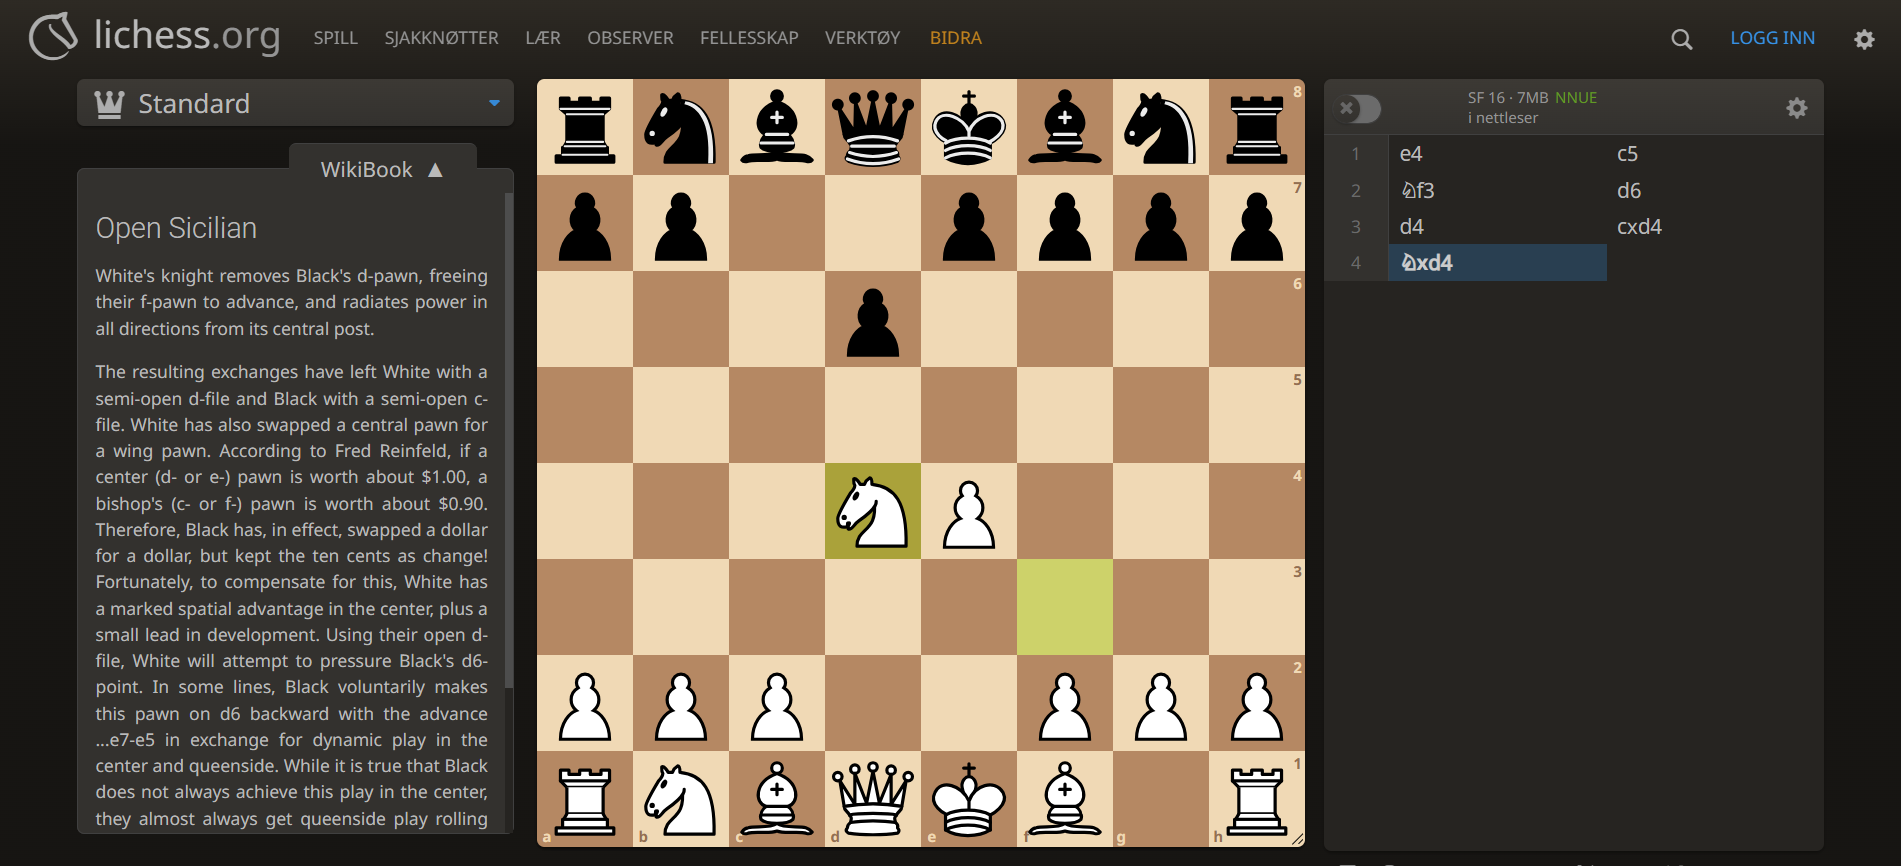
\includegraphics[width=0.75\linewidth]{figures/results/frontend/download-pgn/lichess-analysis.png}}\caption[Lichess analysis tool]{A demonstration of importing a PGN file into Lichess' analysis tool}\label{fig:downloaded-pgn-analysis} \end{figure}

By enabling \gls{pgn} downloads, the system provides users with a convenient way to review games and improve their understanding of chess. Instead of building a custom in-app analysis feature, this solution leverages existing, well-established services that offer robust and detailed feedback. This decision reduces development complexity while still providing users with valuable insights. \\

However, one limitation is that users must leave the application to analyze the game, which can disrupt the user experience slightly. Despite this, integrating \gls{pgn} downloads remains a practical and effective solution, offering immediate access to game data without requiring additional implementation of complex analytical features.

\subsection{Lighthouse Tests}
The frontend application was developed based on wireframes, team discussions, and user testing. To evaluate the quality of the user interface, Lighthouse tests were conducted on every page, with particular focus on the accessibility score. \\

Initial accessibility scores ranged from 80 to 90 across the various pages. To improve these scores, several adjustments were required—primarily involving color contrast. As shown in \ref{subsec:results-color-palette}, a specific color palette was selected for the application. However, issues were identified with the contrast between the primary blue color and the white background in light mode, as well as between the secondary blue (used for buttons) and the black background in dark mode. \\

To address these issues, slightly modified color variants were chosen for each theme. This led to the adoption of a more customized color palette for both light and dark modes. As a result, the application now achieves a 100 accessibility scores throughout all pages, with both light and dark mode. 

\section{Project management}
\label{sec:discussion-project-management}

\section{Challenges}
In addition to ideas for future development, there were also a few obstacles encountered during the development phase of this project. These challenges were addressed as they occurred, and solutions were implemented as part of the final application. \\

\subsection{Camera}
During the development and testing phase of the front-end application, an obstacle related to camera initialization was encountered. The application is designed to access an external USB camera by specifying a camera ID other than 0, since ID 0 typically corresponds to the system's default or built-in (dashboard) camera, which is not relevant to this project.\\

Two identical external webcams were used for this project, both connected via a USB hub. One of the cameras functioned correctly. When connected, the front-end application successfully initialized the camera feed, and the video stream was displayed on the webpage as expected.\\

However, the second camera, did not behave as expected. Despite being physically identical to the first camera and verified to work through the system's built-in camera application, the front-end application failed to display its video feed. Instead, it defaulted to camera ID 0, resulting in the system's dashboard camera being selected.\\

This issue was traced back to a cached or “ghost” device entry in the Windows Device Manager. A ghost device refers to a previously connected hardware device that is no longer physically attached to the system but whose configuration and driver information remain cached by the operating system. These leftover entries can lead to conflicts or incorrect device indexing when similar hardware is reconnected, especially when multiple identical devices are used. In this case, the system appeared to retain prior camera associations, which caused the application to misidentify or incorrectly assign the camera index.

\subsection{Special moves}
When a move is made, the front-end highlights the previous and current tiles of the moved piece. User testing with different color palettes resulted in the selection of a bright contrast color relative to the main design scheme to ensure good visibility. \\

The chessboard component manages the rules of chess, while the front-end is responsible only for storing tile positions and applying styling. In standard moves, highlighting the starting and ending tiles is sufficient. However, special moves such as \gls{castling}, pawn \gls{promotion}, and \gls{en-passant} capture require additional handling. \\

In \gls{castling}, both the king and a rook move simultaneously. Since the default highlight logic tracks only one piece, it does not correctly represent \gls{castling} moves. Additional logic was implemented to highlight the movements of both the king and rook during \gls{castling}, ensuring consistency and clarity for the user.


% Ting som nevnes andre steder i dokumentet som er flyttet hit fordi det funker bedre i diskusjon


%The ONNX format was chosen because it was framework-agnostic, making integration into different deployment environments easier.

%Metode



%(Metode, agile methodology)

%This approach supported shared decision-making and maintained consistency across the project.

%This allowed the team to identify challenges, recognize what worked well, and suggest improvements for future sprints, promoting continuous learning and better teamwork.

%"Status reports involved setting specific sprint goals, outlining the tasks each team member aimed to complete before the next meeting. These meetings also included a review of completed tasks, allowing the team to assess progress and discuss the outcomes of the previous sprint. If any tasks remained incomplete, the team identified potential causes and developed strategies to address them moving forward."

%"Retrospectives provided a chance to reflect on the team's collaboration, discussing both strengths and weaknesses in teamwork."

%"This approach supported shared decision-making and maintained consistency across the project."

%(Metode, User-Centered Design)

%This encouraged honest, unfiltered responses, reducing the likelihood of social desirability bias.

\section{Further Development}
Throughout the project, various development ideas emerged from the team, the product owner, and external contributors. Due to time constraints, these were not implemented and were instead noted as "Further development." At the product owner's request, the focus was on achieving accurate piece recognition over additional features.

\subsection{Independent Application}
During a meeting at Aalesund Schaklag, the product owner and club leader discussed deploying a finalized version of the application with ceiling-mounted cameras. Since the club maintains a standard table layout, the cameras could remain fixed and connected to a computer running the application continuously. A physical switch would allow easy power control.

In a typical use case, the organizer could start an unofficial tournament by turning on the switch, prompting the system to begin tracking games automatically. Once games were finished, the organizer would reset the  returned to their initial position would be recognized as reset. The system would be user-friendly, requiring no technical knowledge and would also protect equipment by having cameras out of reach.

\subsection{Information About Participants}
Currently, all tournament participants are hardcoded into the system. This approach limits scalability and increases the complexity of system maintenance. A more sustainable solution would involve integrating the system with established platforms such as TournamentService, a widely used tool for managing player registration in chess tournaments. \\

TournamentService retrieves player data from both the Norwegian Chess Federation (NSF) and the international FIDE database, ensuring that participant information is accurate and up-to-date.
By implementing such an integration, participants would be able to register by simply searching for their name. The system could then automatically retrieve and populate essential details, such as chess rating, club affiliation, and other relevant metadata. This would significantly streamline the registration process and reduce the likelihood of manual entry errors. \\


\subsection{Time Control}
In chess tournaments, different time formats such as \gls{classical}, \gls{rapid}, and \gls{blitz} are commonly used. The current application does not show time control information, making it harder for spectators to follow the games. Displaying the time control format and countdown timer could enhance the spectator experience. \\

One potential solution is to estimate the remaining time based on move detection. When the machine learning model registers a move, it assumes the player has pressed the clock and that the opponent’s time has begun. However, this method is unreliable due to potential delays in move detection which can lead to inaccurate time tracking. \\

One alternative is using digital clocks with USB connectivity. This method ensures precise and accurate time tracking, as the clock is directly connected to the PC. Digital clocks with \gls{usb}-support such as the DGT3000 offer reliable tracking as the connection ensures the time matches the actual clock. However, these clocks are costly, priced approximately 1000 NOK each \cite{sjakkbutikken:dgt-clock}. Given that Aalesunds Schaklag aims to minimize expenses, this option may not be ideal despite the accuracy it provides. \\

A more affordable but challenging solution is using cameras to visually read physical clocks through a \gls{ml} model. Challenges such as occlusion, poor lighting, and camera resolution make this difficult, especially for faster time controls. \\

Therefore, time control features were not prioritized in the current version but remain an area for future improvement.

\subsection{Multi-Board Detection Capability}
The current system architecture supports a one-to-one mapping between cameras and chessboards, each board requires a dedicated camera. While this setup is functional, it introduces scalability and logistical challenges, particularly in larger tournament settings where numerous boards are involved. \\

Further development could focus on enabling a single camera to detect and track multiple boards simultaneously. This enhancement would significantly reduce the hardware requirements and simplify the setup process, addressing common issues such as cable clutter. \\

Feedback from external collaborators has indicated strong interest in this feature, suggesting it would increase the system's appeal and usability. Implementing multi-board detection would require advances in computer vision algorithms, potentially leveraging techniques such as object detection, perspective correction, and spatial segmentation to reliably differentiate and monitor several boards within a single frame.

\subsection{User-Friendly Variant Selection}
The current version of the application supports different starting positions, but the process for selecting a variant is not user-friendly. While both the backend and frontend are capable of handling non-standard setups, users must manually modify the code to change the game mode. This involves locating the desired variant, copying its \gls{fen} string, and updating it in both the backend and frontend separately, an approach that is not practical for general users. \\

To improve usability, one idea is to implement a user interface that allows players to select from a list of predefined chess variants, each linked to its corresponding \gls{fen} string. This would eliminate the need for manual code changes and make variant selection accessible to all users, enabling broader support for formats such as \textit{\gls{chess960}}, \textit{\gls{horde}}, and \textit{\gls{racing-kings}}.

\subsection{Internationalization}
Currently, the application supports only the English language. Feedback from the usability testing revealed a clear demand for multilingual support, particularly for Norwegian. Several participants noted that not all users are fluent or comfortable with English, which may hinder accessibility and user experience—especially among older users or those less familiar with technical environments. \\

Introducing internationalization (i18n) would make the application more inclusive and accessible to a broader audience. This would involve implementing a localization framework to support multiple language files, enabling dynamic language switching, and ensuring that all UI text elements are properly translatable. \\

As the system is intended for public and possibly international use in tournament settings, multilingual support would be a valuable enhancement. Future development should prioritize adding language selection functionality, beginning with Norwegian, and designing the system architecture to support additional languages as needed.
